\documentclass{beamer}
\usetheme{Madrid}
\usepackage{tikz}
\definecolor{aggiemaroon}{HTML}{500000}
\newcommand{\myplot}[1]{\textbf{Plot of #1}}

\title{Introduction to Machine Learning}
\subtitle{Lecture 1}
\author{Dr. Example}
\institute{Texas A\&M University}
\date{Fall 2026}

\begin{document}

\begin{frame}
  \titlepage
\end{frame}

% \begin{frame}{This frame is commented out and must be ignored}
% \end{frame}

\begin{frame}{Course Logistics}
  \begin{itemize}
    \item Grading: 40\% exams, 60\% projects
    \item<2-> Late work costs \$5 per day % trailing comment
    \item<2-> Office hours:
      \begin{enumerate}
        \item Monday
        \item Thursday
      \end{enumerate}
  \end{itemize}
\end{frame}

\begin{frame}
  \frametitle{Linear Models}
  A model predicts $\hat{y} = w^\top x + b$ from the features.
  \pause
  \[
    L(w) = \frac{1}{n}\sum_{i=1}^{n} \left(y_i - w^\top x_i\right)^2
  \]
  \begin{center}
    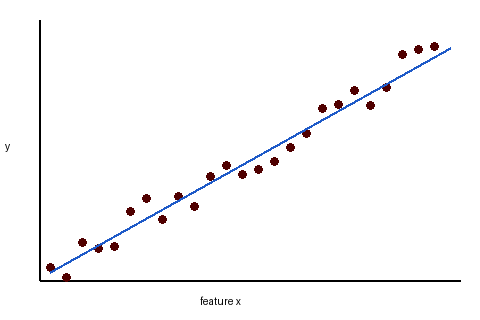
\includegraphics[width=0.45\textwidth]{figs/regression}
  \end{center}
\end{frame}

\begin{frame}{Cross-Validation}
  \begin{itemize}
    \item Split the data into $k$ equal folds
    \item Train on $k-1$ folds, test on the remaining one
  \end{itemize}
  \pause
  \begin{center}
  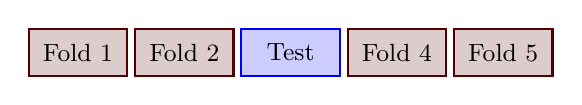
\begin{tikzpicture}
    \foreach \i in {0,...,4}{
      \pgfmathsetmacro{\x}{\i*1.35}
      \draw[fill=aggiemaroon!20, draw=aggiemaroon, thick] (\x,0) rectangle ++(1.25,0.6);
      \pgfmathtruncatemacro{\n}{\i+1}
      \node at (\x+0.625,0.3) {\small Fold \n};
    }
    % the test box is drawn ON TOP of fold 3 and hides its label
    \draw[fill=blue!20, draw=blue, thick] (2.7,0) rectangle ++(1.25,0.6);
    \node at (3.325,0.3) {\small Test};
  \end{tikzpicture}

  \vspace{0.4em}
  {\small One fold is used for testing; the others are used for training.}
  \end{center}
\end{frame}

\begin{frame}{Overlays That Replace Content}
  \only<1>{Step one: collect the data.}
  \only<2>{Step two: clean the data.}
\end{frame}

\begin{frame}{A Custom Macro}
  \myplot{results.csv}
\end{frame}

\end{document}
